\section{Experiment}
In this experiment, a voltage source will be used to provide a range of forward voltages to the LEDs, while a current measurement device will record the corresponding forward currents. By plotting the current-voltage data and analyzing the linear portion of the curve, we can obtain the slope of the line, which is directly related to Planck's constant.

Understanding the value of Planck's constant is crucial for numerous applications, including the development of advanced electronic devices, semiconductor physics research, and the advancement of energy-efficient lighting technologies. By conducting this experiment and determining Planck's constant based on the current-voltage characteristics of LEDs, we can deepen our understanding of quantum mechanics and its practical implications.
\subsection{Formulas}
\large
\begin{itemize}
\item \begin{equation*}
	\Delta X = \frac{a}{100\%} \cdot X + n \cdot \Delta_{res}
\end{equation*}
\item \begin{equation*}
	U_b = - \frac{b}{a} 
\end{equation*}

\item \begin{equation*}
	h = \frac{e}{c}\lambda U_b
\end{equation*}
\item \begin{equation*}
	u_c(U_b) = \sqrt{(b/a^2)^2 \cdot u(a)^2 + (-1/a)^2 \cdot u(b)^2}
\end{equation*}

\item \begin{equation*}
	u_c(h) = \sqrt{(\frac{e}{c} U_b)^2 \cdot u(\lambda)^2 + (\frac{e}{c} \lambda )^2 \cdot u(U_b)^2}
\end{equation*}
\end{itemize} 

e - elementary charge \\
c - velocity of light in vacuum \\
$\lambda$ - wavelength \\
$U_b$ - potential barrier \\
h - Planck constant \\
\subsection*{Data}

\subsubsection*{Initial data}
\begin{table}[H]
    \centering
    \begin{tabular}{l|l|l}
        ~ & V [V]  & I [mA] \\ \hline
        min & 2.53 & 0 \\ \hline 
        max & 3.27 & 16.44 \\ \hline
        ~ & 3.26 & 16.05 \\ 
        ~ & 3.25 & 15.25 \\ 
        ~ & 3.24 & 14.99 \\ 
        ~ & 3.23 & 14.57 \\ 
        ~ & 3.22 & 14.08 \\ 
        ~ & 3.21 & 13.58 \\ 
        ~ & 3.2 & 13.05 \\ 
        ~ & 3.19 & 12.48 \\ 
        ~ & 3.18 & 12.03 \\ 
        ~ & 3.17 & 11.41 \\ 
        ~ & 3.11 & 8.75 \\ 
        ~ & 3.05 & 6.44 \\ 
        ~ & 2.99 & 4.52 \\ 
        ~ & 2.93 & 2.93 \\ 
        ~ & 2.87 & 1.8 \\ 
        ~ & 2.81 & 0.95 \\ 
        ~ & 2.75 & 0.4 \\ 
        ~ & 2.69 & 0.17 \\ 
        ~ & 2.62 & 0.05 \\ 
        ~& 2.56 & 0.01 \\ 
    \end{tabular}
    \caption{Experiment data}
\end{table}


\begin{figure}[H]
	\centering
	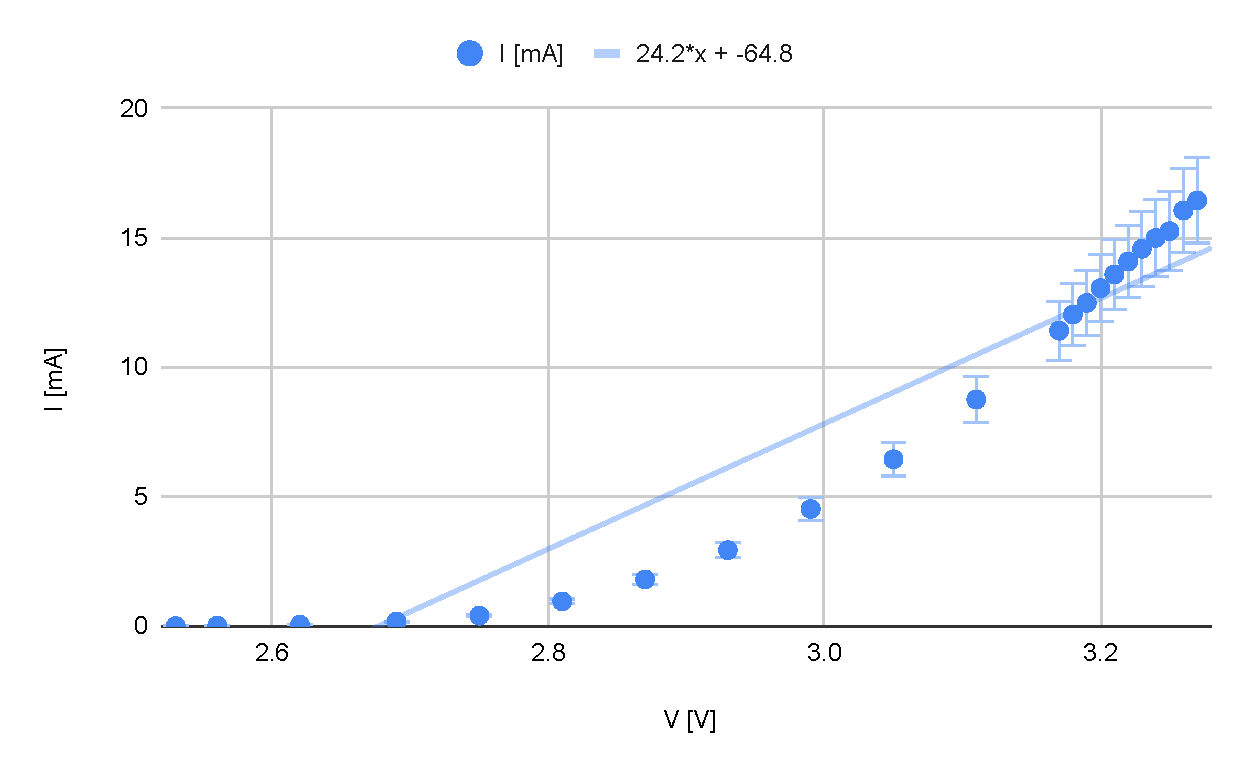
\includegraphics[width=12cm]{schematics/chart.pdf}
	\caption{Current-voltage characteristics}
	
\end{figure}

\begin{table}[H]
	\centering
	\begin{tabular}{l|l|l|l}
		a & u(a)& b  & u(b) \\ \hline
		24.2 & 1.77 & -64.8 & 5.33
		
	\end{tabular}
	\caption{Data obtained from linear regression}
\end{table}

\subsubsection*{Meters Uncertainties}
\begin{table}[!ht]
    \centering
    \begin{tabular}{l|l|l|l}
        $\Delta_p $ & $\lambda$  & I &  U  \\ \hline
        ~ & 10mm & 1.4\% rdg + 3dgt & 0.5\% rdg + 1 dgt \\ 
    \end{tabular}
    \caption{Meters Manual Data}
\end{table}

\subsubsection*{Analysis of results}
\begin{table}[H]
    \centering
    \begin{tabular}{l|l|l|l|l}
        V [V]  & u(V) [V] & I [mA] & u(I) [mA] & $\lambda [nm]$ \\ \hline
        2.53 & 0.02265 & 0 & 0.03 & 466 \\ 
        3.27 & 0.02635 & 16.44 & 0.26016 & 465 \\ 
        3.26 & 0.0263 & 16.05 & 0.2547 & 464 \\ 
        3.25 & 0.02625 & 15.25 & 0.2435 & 466 \\ 
        3.24 & 0.0262 & 14.99 & 0.23986 & 465 \\ 
        3.23 & 0.02615 & 14.57 & 0.23398 &  \\ 
        3.22 & 0.0261 & 14.08 & 0.22712 & ~ \\ 
        3.21 & 0.02605 & 13.58 & 0.22012 & ~ \\ 
        3.2 & 0.026 & 13.05 & 0.2127 & ~ \\ 
        3.19 & 0.02595 & 12.48 & 0.20472 & ~ \\ 
        3.18 & 0.0259 & 12.03 & 0.19842 & ~ \\ 
        3.17 & 0.02585 & 11.41 & 0.18974 & ~ \\ 
        3.11 & 0.02555 & 8.75 & 0.1525 & ~ \\ 
        3.05 & 0.02525 & 6.44 & 0.12016 & ~ \\ 
        2.99 & 0.02495 & 4.52 & 0.09328 & ~ \\ 
        2.93 & 0.02465 & 2.93 & 0.07102 & ~ \\ 
        2.87 & 0.02435 & 1.8 & 0.0552 & ~ \\ 
        2.81 & 0.02405 & 0.95 & 0.0433 & ~ \\ 
        2.75 & 0.02375 & 0.4 & 0.0356 & ~ \\ 
        2.69 & 0.02345 & 0.17 & 0.03238 & ~ \\ 
        2.62 & 0.0231 & 0.05 & 0.0307 & ~ \\ 
        2.56 & 0.0228 & 0.01 & 0.03014 & . \\ 
    \end{tabular}
    \caption{Final data}
\end{table}

\begin{table}[H]
    \centering
    \begin{tabular}{l|l|l|l|l|l}
        $\lambda$ [nm] & u($\lambda$) [nm] & Ub [V] & $u_c(Ub)$ [V] & h [J s] & $u_c$(h) [J s] \\ \hline
        465.2 & 5.8 & 2.7 & 0.3 & 6.66E-34 & $\approx 0$ \\ 
    \end{tabular}
    \caption{Final data}
\end{table}

\subsubsection*{Example calculations:}


\begin{itemize}

\item \begin{equation*}
	u(U) = \frac{a}{100\%} \cdot X + n \cdot \Delta_{res} = 
	(0.5/100) \cdot 2.53 + 1 \cdot 0.01 = 0.03 
\end{equation*}
\item \begin{equation*}
	U_b = - \frac{b}{a} = - \frac{-64.8}{24.2} = 2.68
\end{equation*}

\item \begin{equation*}
	h = \frac{e}{c}\lambda U_b = \frac{1.60E-19}{299792458} \cdot 465.2 
	\cdot 2.68 = 6.66E-34
\end{equation*}
\item \begin{equation*}
	u_c(h) = \sqrt{(\frac{e}{c} U_b)^2 \cdot u(\lambda)^2 + (\frac{e}{c} \lambda )^2 \cdot u(U_b)^2} \approx 0
\end{equation*}
\item values are to small and calculator can't calculate the uncertainty for
$u_c(h)$
\item 
\begin{equation*}
	u_c(U_b) = \sqrt{(b/a^2)^2 \cdot u(a)^2 + (-1/a)^2 \cdot u(b)^2} =
	0.3
\end{equation*}

\end{itemize}

